\chapter{Obstructed atomic limits and fractional corner charges}
\label{ch:oals}


\section{Crystal symmetries}
Gapless boundary modes in topological crystalline insulators are protected by spatial symmetries which act non-locally (i.e. mirror symmetry $M_z: x \rightarrow -x$
Prediction of 3D TCI with two-dimensional surface states in the semiconducting SnTe protected by the mirror symmetry~\cite{FuTCI2011, HsiehTCI2012}.

Extending the classification schemes to crystal symmetries ~\cite{Slager2013, PhysRevB.90.165114, PhysRevB.93.195413, PhysRevB.95.235425, PhysRevB.93.045429}.

Crystal symmetries give rise to a generalization of TIs called higher-order topological insulators, where non-trivial $d$-dimensional bulk is accompanied by boundary modes in less than $(d-1)$-dimensions~\cite{Benalcazar61, PhysRevLett.119.246401, HOTI12018}. For instance, 3D system may exhibit 1D hinge modes/


A general framework of topological quantum chemistry~\cite{TQC2017}

\section{Modern theory of polarization: Wannier functions}
Those systems can be understood using the Wannier functions. Given a set of occupied Bloch states, one may construct the Wannier function as their Fourier transform:
\begin{equation}
\ket{\mathbf{R} n} = \frac{V}{(2 \pi)^3} \int_{BZ} d \mathbf{k} e^{i \mathbf{k} \cdot \mathbf{R}} \sum_{m = 1}^J U_{mn} (\mathbf{k}) \ket{\psi_{m\mathbf{k}}} 
\end{equation}
In general, Wannier functions are not uniquely defined, only the sum over the Wannier centers in a given unit cell. Most often, the rotation matrix $U_{nm}$ is determined in such a way the minimizes the spread in a real space (= the sum of the mean squares) of the Wannier function. For more detailed discussion, we refer to the review by Marziari \emph{et al.}~\cite{MarziariWF2012}. 

Obstructed atomic limits admit the Wannier function representation, (with Wannier functions being exponentially localized and symmetry-preserving) which is in contrast to strong topological phases. However, the Wannier centers do not coincide with atomic positions (as in the case of trivial atomic limit), but they are rather localized on other symmetric points in the unit cell called the Wyckoff positions.


\begin{figure}
\centering
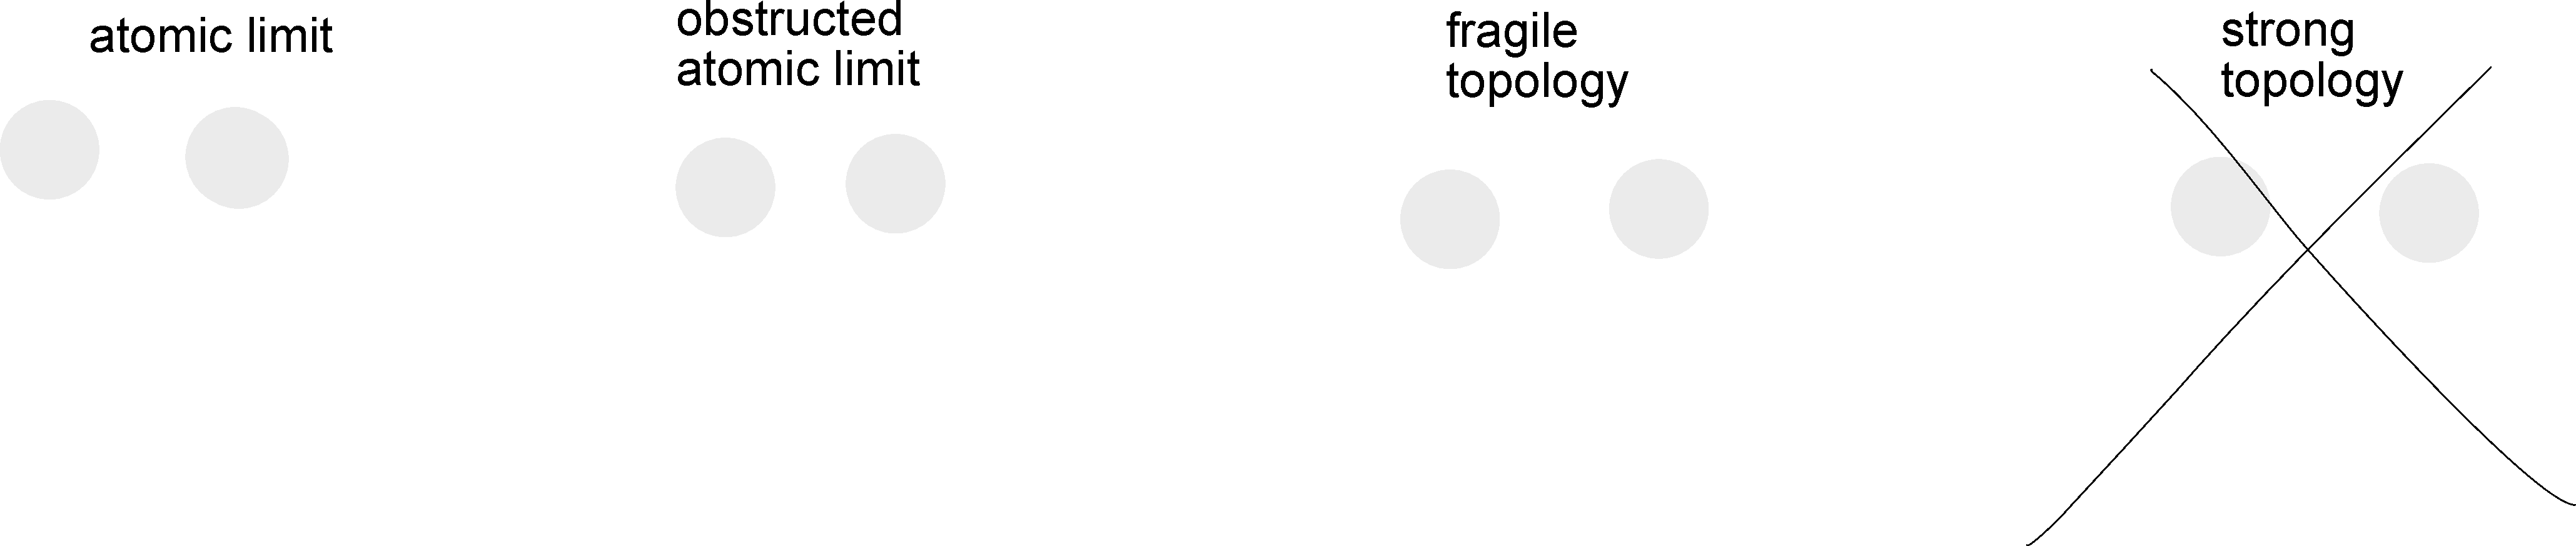
\includegraphics[width=\columnwidth]{oal_newphases}
\caption{In the presence of crystal symmetries, a distinction between topological and trivial phases is less pronounced. Atomic limit corresponds to the situation where Wannier charge centers are located on atomic positions. In case of obstructed atomic limits, Wannier functions are exponentially localized on the Wyckoff positions. Fragile phases cannot be represented in terms of Wannier functions, but a strong index vanishes. Strong topological phases (such as TI or CI) do not admit Wannier representation.}
\label{fig:newphases}
\end{figure}






Note that the charge fractionalization mechanism is different that in, for example, spin liquids. Here it's due to cutting Wannier functions in a finite sample.




\section{Bulk indices}
The key goal was to construct the bulk indices for all layer groups to be sure that boundary effects are related to the nontrivial bulk rather than suitable edge termination.



\subsection{Symmetry indicators}
Fu-Kane formula presented in Chapter~\ref{ch:topo-intro} was actually the first symmetry indicator. In a similar manner, one may construct the quantities which will count


\subsection{Wilson loops}

Given the projector onto occupied states $P:= \sum_{E < E_F} \ket{\psi} \bra{\psi}$, the Wilson loop is defined as a product of $P$ along closed path $\gamma$ in $k$-space:
\begin{equation}
W_{\gamma} = \prod_{\mathbf{k}} P ( \mathbf{k}) 
\label{eq:wilson}
\end{equation}
and it is gauge invariant.

\section{Material candidates}
Predicted also in atomically thin carbon allotrope called graphdiyne~\cite{GDY12019, GDY22019}.


As potential experimental realization, we propose group-V honeycomb monolayers of bismuth, antimony and arsenic. They share the very same crystal structure. With non-zero buckling, these systems preserve $C_3$ and $\mathcal{I}$. When $d_z = 0$, TCI phase is exhibited.


\begin{figure}
\centering
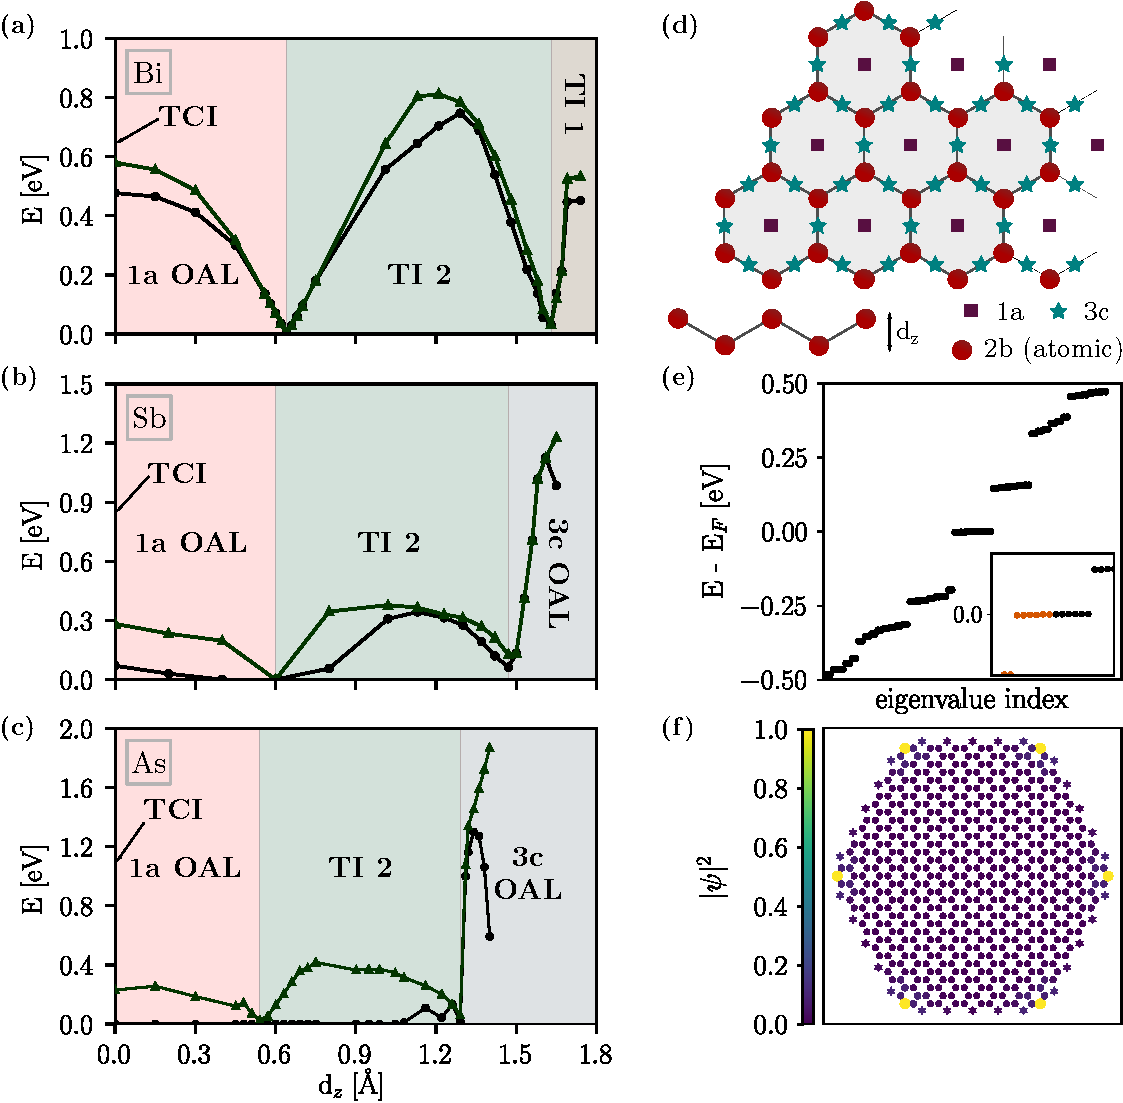
\includegraphics[width=\columnwidth]{oal_finite}
\caption{Low-energy spectrum of a finite armchair-terminated flakeof the 3cOAL. The inset presents the energies around the Fermi level, with filled states in orange. (f) The electronic densities of the cornerstates with color scale proportional to the normalized square modulus of the eigenstates $|\psi|^2$ (normalized with respect to the largest $|\psi|^2$).The tellurium atoms used for edge passivation are shown as stars.}
\label{fig:oal_finite}
\end{figure}


In Fig.~\ref{fig:oal_finite} we show
